\documentclass[12pt]{article}
\usepackage{../preamble}
\graphicspath{{pics/hw1/}}
\begin{document}
% \maketitle
\chead{Model workshop pre-notes}

%%%%%%%%%%%%%%%%%%%%%%%%%%%%%%%%%%%%%%%%%%%%%%%
%                  Definitions                %
%%%%%%%%%%%%%%%%%%%%%%%%%%%%%%%%%%%%%%%%%%%%%%%
%\includegraphics[width=\mywidth\textwidth]{}

% \begin{figure}[h!]
% \centering
% \input{pics/PS2/p7b}
% \caption{}
% \label{fig-}
% \end{figure}

% \begin{enumerate}[label=\alph*.]
%     \setcounter{enumi}{1}
%     \item 
% \end{enumerate}

%%%%%%%%%%%%%%%%%
%     Part a    %
%%%%%%%%%%%%%%%%%


%%%%%%%%%%%%%%%%%%%%%%%%%%%%%%%%%%%%%%%%%%%%%%%
%                Problem 1                    %
%%%%%%%%%%%%%%%%%%%%%%%%%%%%%%%%%%%%%%%%%%%%%%%
\problem{Subsidizing cleaner products}{
\begin{itemize}
    \item Fixed gov't revenue $R$
    \item Want to subsidize adoption of new class of cleaner products. Multiple products on the market.
\end{itemize}

\textbf{Goal:} want to maximize total quantity of product sold while keeping in mind equity concerns with who is receiving the benefit of the subsidy.\\

\textbf{We have:}
\begin{itemize}
    \item Estimated demand for products in this class (with cleaner tech.)
    \item Demand est. separately for each product and by demographic group (e.g., income)
\end{itemize}\vspace{1em}

\textbf{Focus of paper:}
\begin{itemize}
    \item Theory model
    \item Demand estimates
    \item Policy simulations that use demand estimates to shed light on theory
\end{itemize}\vspace{1em}

\textbf{Model:} should give principles for how subsidies should be structured to maximize diffusion of cleaner products.
}

To develop concepts, I'm going to start with a simple model, modified slightly from Sarah Armitage's JMP\footnote{Armitage, Sarah. “Technology Adoption and the Timing of Environmental Policy: Evidence from Efficient Lighting.” Job Market Paper, November 14, 2021. \url{https://scholar.harvard.edu/files/sarmitage/files/armitage_jmp_harvard.pdf}.}, where the demand estimation is a modification of the BLP-style discrete choice modeling.\footnote{Berry, Steven, James Levinsohn, and Ariel Pakes. “Automobile Prices in Market Equilibrium.” Econometrica 63, no. 4 (1995): 841–90. \url{https://doi.org/10.2307/2171802}.} I also use Nevo (2000) as a helpful guide.\footnote{Nevo, Aviv. “A Practitioner’s Guide to Estimation of Random-Coefficients Logit Models of Demand.” Journal of Economics \& Management Strategy 9, no. 4 (Winter 2000): 513–48. \url{https://doi.org/10.1162/105864000567954}.} While I wanted to start with a 1 period model below for simplicity to understand the situation, I think an important considering is inter-temporal substitution among different cleaner products -- this is what Armitage's method is useful for.

\def\D{\boldsymbol{D_i}}
\def\x{\boldsymbol{x_{jt}}}
\def\p{\boldsymbol{p_{jt}}}
\def\c{\boldsymbol{\xi_{jt}}}
\def\U{U_{ijt}}
\def\b{\boldsymbol{\beta}}
\def\sumi{\sum\limits_i} 
\def\sumj{\sum\limits_j}
\def\sumk{\sum\limits_k}
\textbf{Setup:}
\begin{itemize}
    \item Start with static model -- 1 period
    \item This is a nice setup for discrete choice since many consumer products that policy makers may want to incentivize are large appliances that you would only buy one of.
    \item product $j\in J$ in market $t\in T$, with observed \& unobserved product characteristics $\x$, $\c$
    \item consumer $i\in I_t$, with vector of demographics $\D$
    \item Indirect utility for individual $i$ purchasing one unit of product $j$ in market $t$:\\
    $\U=\x\b  - \alpha\p +\c+ [-\p\quad \x]\cdot(\Pi \D +\Sigma\nu_i) + \varepsilon_{ijt}$\\
    $\p$ market price (can be replaced with $\p +t_j$, where $t_j$ is the tax (subsidy) on good $j$) \\
    $\alpha, \b$ all-consumer taste parameters (estimated) \\
    $\Pi$ demographic taste parameters (estimated)\\
    $\Sigma$ idiosyncratic random coefficients
    \item Consumers can also choose the outside option to not purchase any thing this period (and stay with their already-owned dirty good?); utility of outside option normalized to zero.
    \item Only can choose one product in the period.
    \item The products have per-unit externalities $e_j$ such that 
    $e_D > e_{C2} \geq e_{C1} \geq0 $
    \item $Q_j$ = total quantity of good $j$ sold
    \item Gov't budget constraint: $R=\sum_j -t_j Q_j$
    \item Pigouvian prescription would be to set the tax on each good equal to the marginal damages from each good: $\tau_j^*=e_j$
    \item Assume we cannot set a tax on the dirty good. What taxes (subsidies) would we place on the clean goods?
\end{itemize}

\textbf{Proposition 3 from Armitage:} When the social planner is constrained to implement a tax schedule on one clean good
only and there are three goods, the efficient second-best pricing policy on the first clean good is given by

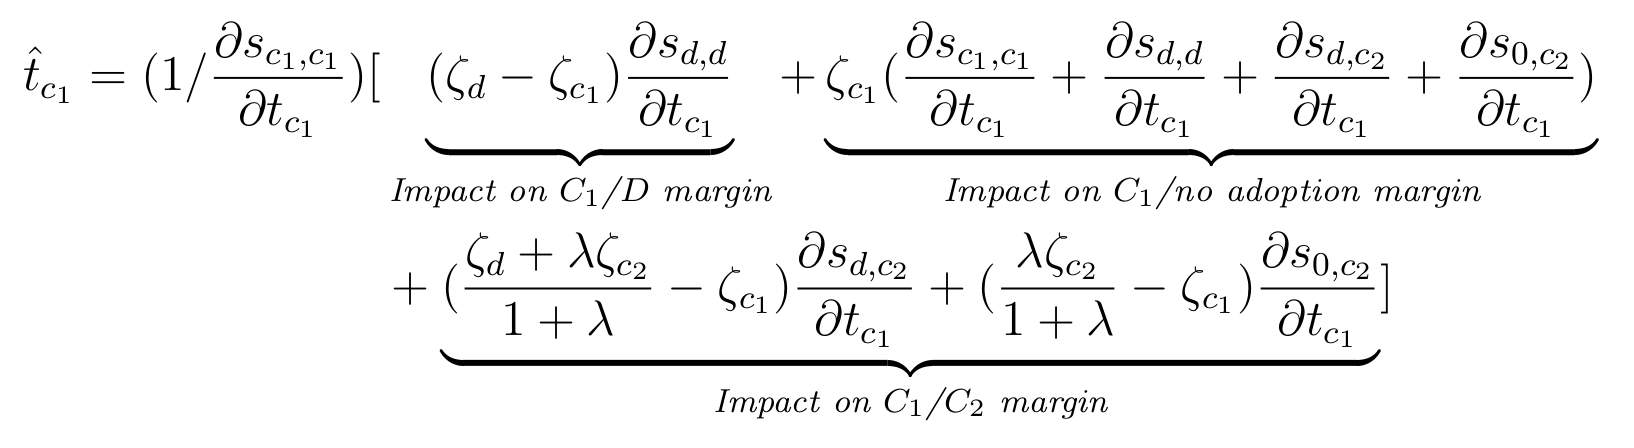
\includegraphics[width=0.9\textwidth]{second-best-taxArmitage}

This is if the $C_2$ good only comes to market after the $C_1$ good has been subsidized. A similar derivation could be used to find the second-best tax on all the clean goods if the dirty good cannot be taxed.

In estimating demand though the BLP framework, we get estimates of the average and demographic-specific price sensitivity ($\alpha$, first row of $\Pi$). We can use these to understand how people will react to the subsidies -- estimating shares of the population, by demographics, that will switch to the different products given a vector of subsidies (negative taxes).

We want to maximize the social welfare function over the choice of subsidies, subject to our revenue $R$ budget constraint. If these second-best optimal subsides show to be regressive, we may choose subsidies that do not achieve this optimum but are more progressive instead.

\textbf{Questions:}
\begin{itemize}
    \item How will subsidizing these different products affect market structure? We probably care about the long-run effects of this (Armitage, 2021)
    \item What does the social welfare function look like?
    \item Separability: could we just use the second-best optimal subsidies using $R-R_1$ of the revenue, and then additionally target $R_1$ funds to giving rebates to specific households under a certain income level?
\end{itemize}


\end{document}

